\begin{multicols}{3}
\byline{Интервю с инж. Виолета Илиева - началник на РИО Бургас}{Карина 
Пазвантова и Гергана Костова, 10Е}

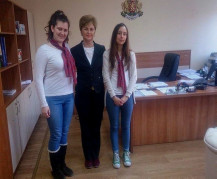
\includegraphics[width=2.1in]{./Ilieva/Ilieva.jpg}

Какво е мнението Ви за новото поколение?

Може би учителската професия е една от най–облагодетелстваните професии, тъй 
като дава възможност на всеки един човек, независимо на каква възраст е, да се 
среща с млади хора. Когато си учтив по цял ден с млади хора и усещаш техния дух, 
техния импулс, неминуемо и ти се потапяш в атмосферата на това младо поколение.

Какво е мнението Ви за мястото на ГПНЕ „Гьоте” в образователното пространство 
на областта?

Безспорно Немската езикова гимназия е едно от училищата, което има завидно 
място, най–вече заради постиженията, които имат учениците, както и възможността 
да получат Шпрахдиплом (Sprachdiplom) Конференцията на министрите на културата 
на Федерална република Германия. От гледна точка на служителите в инспектората е 
много лесно да се прави прием в немската гимназия, тъй като още на първо 
класиране всички места са заети и оттам нататък ангажиментът на инспектората 
отпада. ГПНЕ „Гьоте” присъства и в културния живот на град Бургас. Като започнем 
още от учителите, които са преподавали там, включително и тези, които са 
работили в инспектората като експерти, имам предвид Венда Райкова, поетеси, 
които вземат и заслуженото място в културния живот на град Бургас. Те са 
разпръснали искрицата и любовта към изкуството в Немска езикова гимназия. Още 
преди години на учениците, учещи във вашето училище се правиха препоръки в 
инспектората, за да могат да кандидатстват и да презентират своето творчество в 
други институти извън страната, като отбелязвахме участието им в различни 
литературни конкурси. Не е за подценяване и дейността на Вашето ръководство при 
изграждането на паметника на Гьоте, защото, доколкото знам, само в няколко от 
немските гимназии в страната има изграден подобен паметник. Класирането ви на 
ДЗИ - почти винаги сте в първата десетка както по български език, така и по 
други учебни предмети. Така че, немската езикова гимназия, макар намираща се в 
една сграда с английската гимназия, и често да спорите за физическо 
пространство, духовното пространство на гимназията ви е много голямо.

Имате ли съвместна работа с немската езикова гимназия и в какво се състои тя?

С Немската езикова гимназия ни свързва преди всичко работата по проекти.  В 
момента се реализира  проектът между община Бургас и област Дегендорф. Вашите 
учители ще обучават стажантите, които ще бъдат изпратени в Германия. Но преди да 
заминат там е необходимо тези ученици-стажанти, които се явиха на конкурс и 
които бяха одобрени,  да преминат през езиково обучение за получаване на B1 и 
това ще извършат част от учителите в Немската гимназия.

Каква стратегия има регионалният инспекторат за подкрепа на такива училища 
като нашата гимназия?

В момента знаете, че българското образование е в процес на реформи и това, което 
се прави в училищата, в които има ученици, показали високи резултати на 
национално външно оценяване, както и постигнали резултати на международни 
конкурси и състезания, е към бюджета на училището да има една допълнителна 
добавка за даровити деца, за деца, които показват резултати от учебната дейност 
по-високи от нивото на средния резултат в страната с цел поощряване на таланта, 
което аз подкрепям.

Какво е Вашето пожелание по случай 55 – годишнината на нашата гимназия?

Пожелавам на вашата гимназия още много, много дълги години да продължава да 
привлича таланти, ученици, които са силно мотивирани, така че, всички Вие, които 
завършвате тази гимназия да се реализирате по вашите желани професии и 
специалности, да имате хобита, с които да допринесете за развитието на нашия 
хубав град.
\closearticle
\end{multicols}